\newpage
\thispagestyle{sectioned}
\chapter{Aqtuitectura}

\subsection{Arquitectura de la aplicacción}

La arquitectura está compuesta por tres módulos principales de los que hablaremos en profundidad en las siguientes subsecciones. Como cliente móvil tendremos la aplicación desarrollada en Android, que realizará peticiones HTTP al servicio web alojado en OpenShift, una plataforma que permite alojar servicios web de forma gratuita. Dentro del servicio contaremos con una API RESTful que será quien gestione las peticiones de la aplicación móvil mediante el protocolo HTTP.

\begin{figure}[H]
\centering
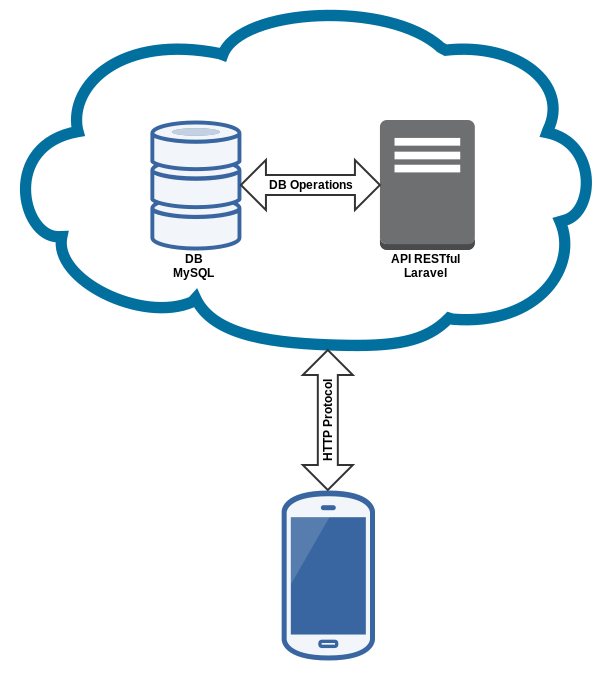
\includegraphics[keepaspectratio, scale=0.4]{Media/Captures/architecture.png}
\caption{Arquitectura de la aplicacción.}
\label{fig:architecture}
\end{figure}

Por último, la base de datos MySQL alojada en el servidor de OpenShift \cite{ref:OpenShift}, almacenará toda la información relacionada con la aplicación. La API RESTful será quien gestione las operaciones de la base de datos.

\subsection{Back-end}

\subsubsection{Base de Datos}\label{sssec:database}
Para la implementación de la base de datos, se ha utilizado un modelo relacional para la definición de las tablas. Utilizando MySQL \cite{ref:MySQL} como sistema de gestión de base de datos phpMyAdmin \cite{ref:phpMyAdmin} como herramienta de gestión gráfica de la base de datos.

La base de datos está formada por un total de 12 tablas donde se almacena toda la información relacionada con los programas de los partidos políticos, las propuestas ciudadanas, encuestas, comparativas, …, y otros datos más técnicos como la gestión de los usuarios, la relación de los comentarios o la relación entre las secciones y comparativas entre otras.

\begin{figure}[H]
\centering
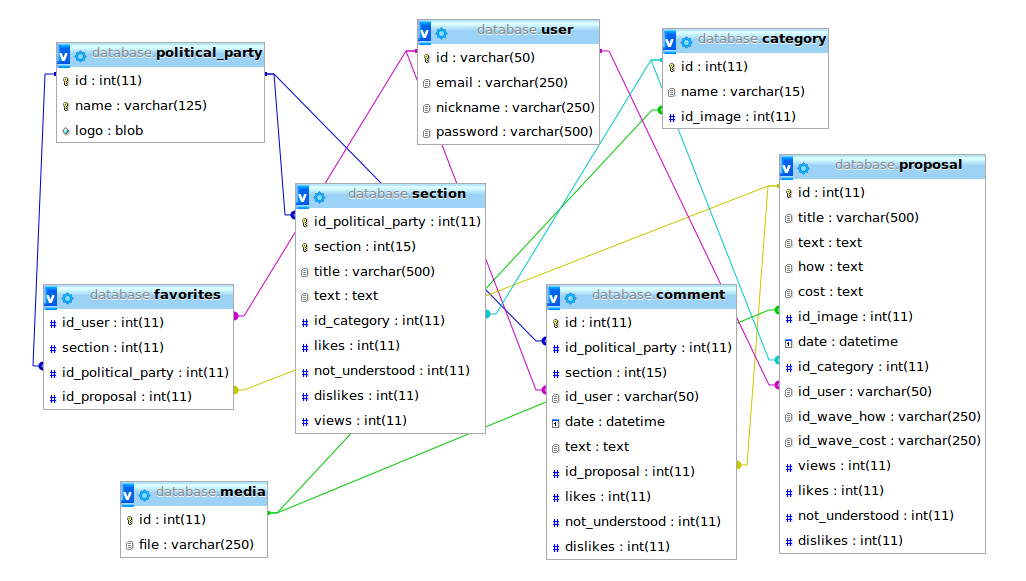
\includegraphics[keepaspectratio, scale=0.30]{Media/Captures/database.png}
\caption{Modelo entidad-relación de la base de datos.}
\label{fig:ermodel}
\end{figure}

Las tablas section y \textit{political-party} son utilizadas para guardar información estática en la aplicación. Es decir, en la tabla \textit{political-party} se almacenan los partidos políticos que se presentan a unas elecciones, y en la tabla \textit{section}, las diferentes secciones de un programa electoral. Tan sólo modificaremos las columnas de \textit{likes}, \textit{dislikes}, \textit{not-understood} y \textit{views} para obtener estadísticas de uso de cada sección. El resto de las columnas permanecerán intactas.

Las demás tablas serán utilizadas para guardar datos dinámicos en la aplicación. Datos que normalmente genera un usuario visitando una sección de un programa, creando una propusta, haciendo un comentario, etc.

\subsubsection{Service REST}\label{sssec:rest}

Para establecer la conexión de la base de datos con la aplicación desarrollada en Android, hemos utilizado Laravel como servicio web. Laravel \cite{ref:laravel}  un framework de código abierto para desarrollar aplicaciones web con PHP 5.

Laravel nos permite montar un sistema de RESTful para que el cliente móvil pueda hacer peticiones al servicio web. Estas peticiones se realizan mediante el protocolo HTTP, en función de la operación que deseemos hacer, haremos una petición GET, POST, PUT, …, etcétera.

\begin{figure}[H]
\centering
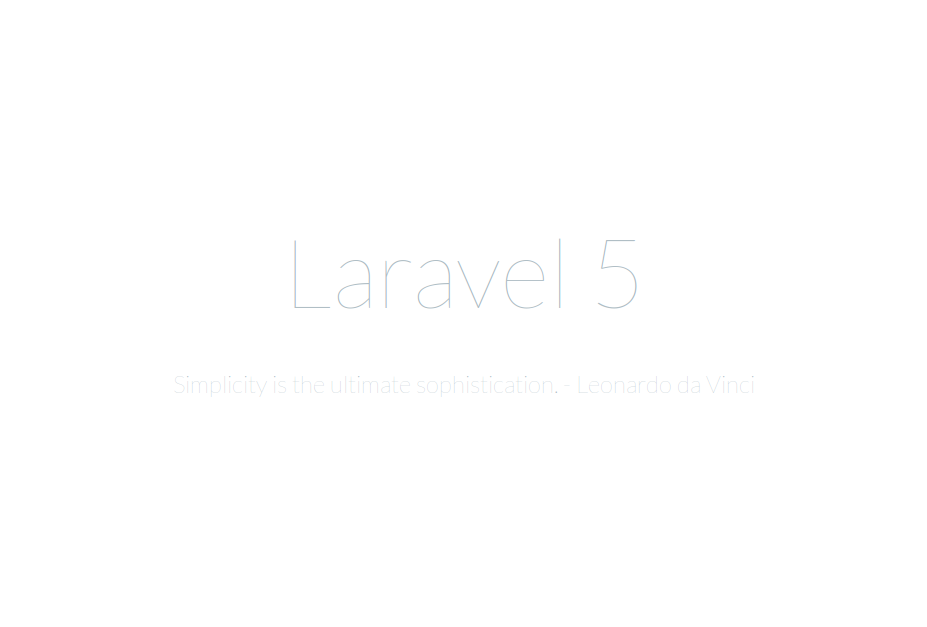
\includegraphics[keepaspectratio, scale=0.30]{Media/Captures/laravel5.png}
\caption{Pantalla principal de Laravel 5.}
\label{fig:laravel5}
\end{figure}

Establecer un servicio RESTful nos proporciona una gran flexibilidad. Pues no solo podremos hacer peticiones desde el cliente en Android, si no que más adelante si pretendemos desarrollar una versión web o incluso un cliente para iOS, las peticiones serán las mismas.

Para organizar las diferentes peticiones en función de su uso y requisitos, Laravel permite montar una API REST (Representational State Transfer), un estilo de arquitectura software para sistemas hipermedia distribuidos como la World Wide Web. Este término se originó en una tesis doctoral sobre la web escrita por Roy Fielding \cite{ref:RESTPhd}.

\subsection{Frontend}